\section{Contextualização da atividade}

A primeira parte da atividade exige que sejam determinados, utilizando o fluxo ótimo de potência linearizado, os seguintes valores de variáveis:
		
		\begin{normalsize}
		\centering

		$\begin{bmatrix}
			P_{G1} & P_{G2} & P_{G3} & \theta{_1} & \theta{_2} & \theta{_3} &
			\lambda{_1} & \lambda{_2} & \lambda{_3} & \lambda{_4}
		\end{bmatrix}$
		
		\end{normalsize}
		
		Estes valores são referentes ao sistema representado na Figura \ref{fig:sist}.
		
		\begin{figure}[!h]
		\centering
		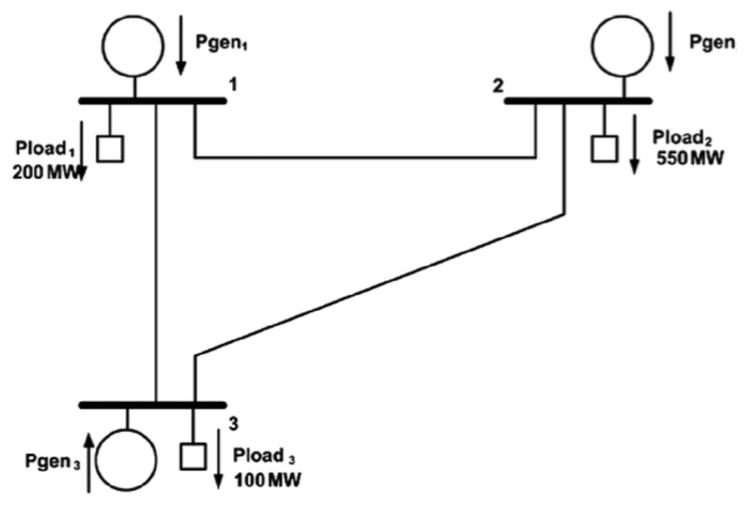
\includegraphics[scale=.3]{sist1}
		\caption{Sistema de três barras}
		\label{fig:sist}
			
		\end{figure}
		
		Para esta análise, será considerado que:
		
		\begin{itemize}
			\item O limite máximo para o fluxo de potência ativa na linha 1-2 seja de $150$ $MW$;
			\item As funções custo para cada gerador são fornecidas pelas Equações \ref{eq:custo1}, \ref{eq:custo2} e \ref{eq:custo3}.
		\end{itemize}
		
		\begin{equation}
			C_1(P_1) = 561 + 7,92*P_1 + 0,001562*P_1^2
			\label{eq:custo1}
		\end{equation}
		
			\begin{equation}
			C_2(P_2) = 310 + 7,85*P_2 + 0,00194*P_2^2
			\label{eq:custo2}
		\end{equation}
		
			\begin{equation}
			C_3(P_3) = 78 + 7,97*P_3 + 0,00482*P_3^2
			\label{eq:custo3}
		\end{equation}
		
		Como informações adicionais, observa-se que a \textbf{barra 1} é adotada como a barra de referência e considera-se uma base de potência de $100$ $MVA$. As reatâncias das linhas estão dispostas conforme a Tabela \ref{tab:reat1}.
		
		
\begin{table}[!h]
\centering
\caption{Reatância das linhas (por unidade)}
\label{tab:reat1}
\begin{tabular}{|c|c|}
\hline
\textbf{Linha} & \textbf{Reatância da linha (p.u.)} \\ \hline
\textit{1-2} & $x_{12}$ = 0,1 \\ \hline
\textit{1-3} & $x_{13}$ = 0,125 \\ \hline
\textit{2-3} & $x_{23}$ = 0,2 \\ \hline
\end{tabular}
\end{table}

\section{Resolução do problema proposto}

	Todos os cálculos referentes a esta solução foram efetuados no \textit{software} MATLAB®
	
	\subsection{Equacionamento e definição de métodos}
	
	A partir do método de determinação do fluxo de potência linearizado, é possível determinar a função restrição a ser utilizada na etapa de otimização.
	
	Dispensando uma explanação extensa, a formulação matricial do estudo de fluxo de potência pelo método linearizado é representado pela expressão:
	
	\begin{equation}
		P = B'*\theta
		\label{eq:res1}
	\end{equation}
	
	Em que:
	
	\begin{itemize}
		\item $P$ = Potência ativa líquida injetada nos nós das barras.
		\item $\theta$ = Ângulos de fases das tensões nas barras.
		\item $B'$ = Matriz admitância nodal.
	\end{itemize}
	
	Com relação a Equação \ref{eq:res1}, entende-se que:
	
	\begin{equation}
		B'*\theta - P = 0
		\label{eq:res2}
	\end{equation}
	
	Sendo assim, a Equação \ref{eq:res2} é a função restrição do sistema a ser otimizado para uma determinada operação, uma vez que o atendimento de todas as cargas deve ser conservado, configurando em uma restrição de igualdade.
	
	Portanto, para cada barra, há uma função restrição $h(P_{Gk},\theta{_{k1}},...,\theta{_{kn}})$ que obedece a seguinte relação:
	
	\begin{equation} %Verificar se há coerência na eq.
		h(P_{Gk},\theta{_{k1}},...,\theta{_{kn}}) = \Bigg(\displaystyle\sum_{k,n=1}^{n=a} B'_{kn}*\theta{_n}\Bigg) - P_k
		\label{eq:res3}
	\end{equation}
	
	Em que, na Equação \ref{eq:res3}, $a$ refere-se ao número de barras do sistema. Neste caso, o número de barras do sistema proposto é \textbf{três}.
	
	Em otimização, o método dos multiplicadores de Lagrange será implementado nesta etapa, uma vez que as funções restrição são bem definidas, conforme apresentado anteriormente pela Equação \ref{eq:res3}.
	
	A formulação genérica de Lagrange é dada pela expressão abaixo:
	
	\begin{equation}
		L(x_1,...,x_n,\lambda{_1},...,\lambda{_n}) = (\text{Funções-objetivo}) + \lambda*(\text{Funções-restrição})
		\label{eq:res4}
 	\end{equation}
 	
 	As funções-objetivo na Equação \ref{eq:res4} são as funções custo apresentadas anteriormente pelas Equações \ref{eq:custo1}, \ref{eq:custo2} e \ref{eq:custo3}. As funções-restrição são as funções resultantes da relação representada na Equação \ref{eq:res3} com relação a restrição de igualdade imposta pela análise do fluxo de potência.
 	
 	
\subsection{Cálculo dos parâmetros}
 	
 	Para a definição da função-restrição do sistema representado pela Figura \ref{fig:sist}, utiliza-se novamente a Equação \ref{eq:res3}.
 	
 	Determina-se a matriz $B'$ com relação a Tabela \ref{tab:reat1}, representada de acordo com a matriz na Expressão \ref{exp:Binc}.
 	
 	\begin{equation}
 		B' = \begin{bmatrix}
 		\frac{1}{0,1}+\frac{1}{0,125} & -\frac{1}{0,1} & -\frac{1}{0,2} \\[0.3em]
       -\frac{1}{0,1} & \frac{1}{0,1}+\frac{1}{0,2} & -\frac{1}{0,2} \\[0.3em]
       -\frac{1}{0,2} & -\frac{1}{0,2} & \frac{1}{0,125}+\frac{1}{0,2}\end{bmatrix}
       \label{exp:Binc}
     \end{equation}
     
     Desta forma, a matriz $B'$ é representada abaixo na Expressão \ref{exp:B}.
     
     \begin{equation}
    	B' = \begin{bmatrix}
       18 & -10 & -8 \\
       -10 & 15 & -5 \\
       -8 & -5 & 13\end{bmatrix}
       \label{exp:B}
		\end{equation}
		
	Com isso, utilizando-se da Equação \ref{eq:res1}, a função-restrição é representada conforme a Equação.
	
	\begin{equation}
		\begin{bmatrix}
       18 & -10 & -8 \\
       -10 & 15 & -5 \\
       -8 & -5 & 13\end{bmatrix} * 
       \begin{bmatrix}
       	\theta{_1} \\
       	\theta{_2} \\
       	\theta{_3} \\
       \end{bmatrix} = 
       \begin{bmatrix}
       	P_{G1} - P_{C1} \\
       	P_{G2} - P_{C2} \\
       	P_{G3} - P_{C3} \\
       \end{bmatrix}
       \label{exp:RES1}
	\end{equation}
 	
 	Ao multiplicar a grandeza por unidade pelo seu valor de base, com a finalidade de se obter os valores de Potência líquida ($P_{G1} - P_{C1}$) em sua unidade real ($MW$), e representar a Equação \ref{exp:RES1} de acordo com a Equação \ref{eq:res4}, obtêm-se a seguinte relação:
 	
 	\begin{equation}
		100*\begin{bmatrix}
       18 & -10 & -8 \\
       -10 & 15 & -5 \\
       -8 & -5 & 13\end{bmatrix} * 
       \begin{bmatrix}
       	\theta{_1} \\
       	\theta{_2} \\
       	\theta{_3} \\
       \end{bmatrix} - 
       \begin{bmatrix}
       	P_{G1} - P_{C1} \\
       	P_{G2} - P_{C2} \\
       	P_{G3} - P_{C3} \\
       \end{bmatrix} = 0
       \label{exp:RES2}
	\end{equation}
	
	skfioakfaskfas
 	
 	
	
	
	
	
	